\subsubsection{Nelder--Mead}

The NM method is a highly popular derivative-free optimisation algorithm, which maintains a set of points $\{y_1, y_2, \cdots, y_{n+1}\}$ during the optimisation, $n$ being the number of parameters being optimised (or the \textit{dimension} of the optimisation problem).
The convex hull of these points, $Y$, is the smallest possible set of points which contains all the $y_k$ and is convex, in that
\begin{equation}
    \label{eq:convex_hull}
    \forall x_1, x_2 \in Y, \forall \alpha \in [0, 1], \alpha x_1 + (1 - \alpha) x_2 \in Y,
\end{equation}
and in this context is called a \textit{simplex}.
If this convex hull is nonempty---or equivalently, if the $n$ vectors $y_k - y_1$ ($2 \leq k \leq n + 1$) are linearly independent---then the simplex is called \textit{nonsingular}.
(To provide an analogy for $n = 2$, the convex hull is the shape obtained by stretching a rubber band around three pins placed at the points $y_1, y_2, y_3$.
The simplex would be singular if the three points were collinear.)

\begin{figure}[htb]
    \centering
    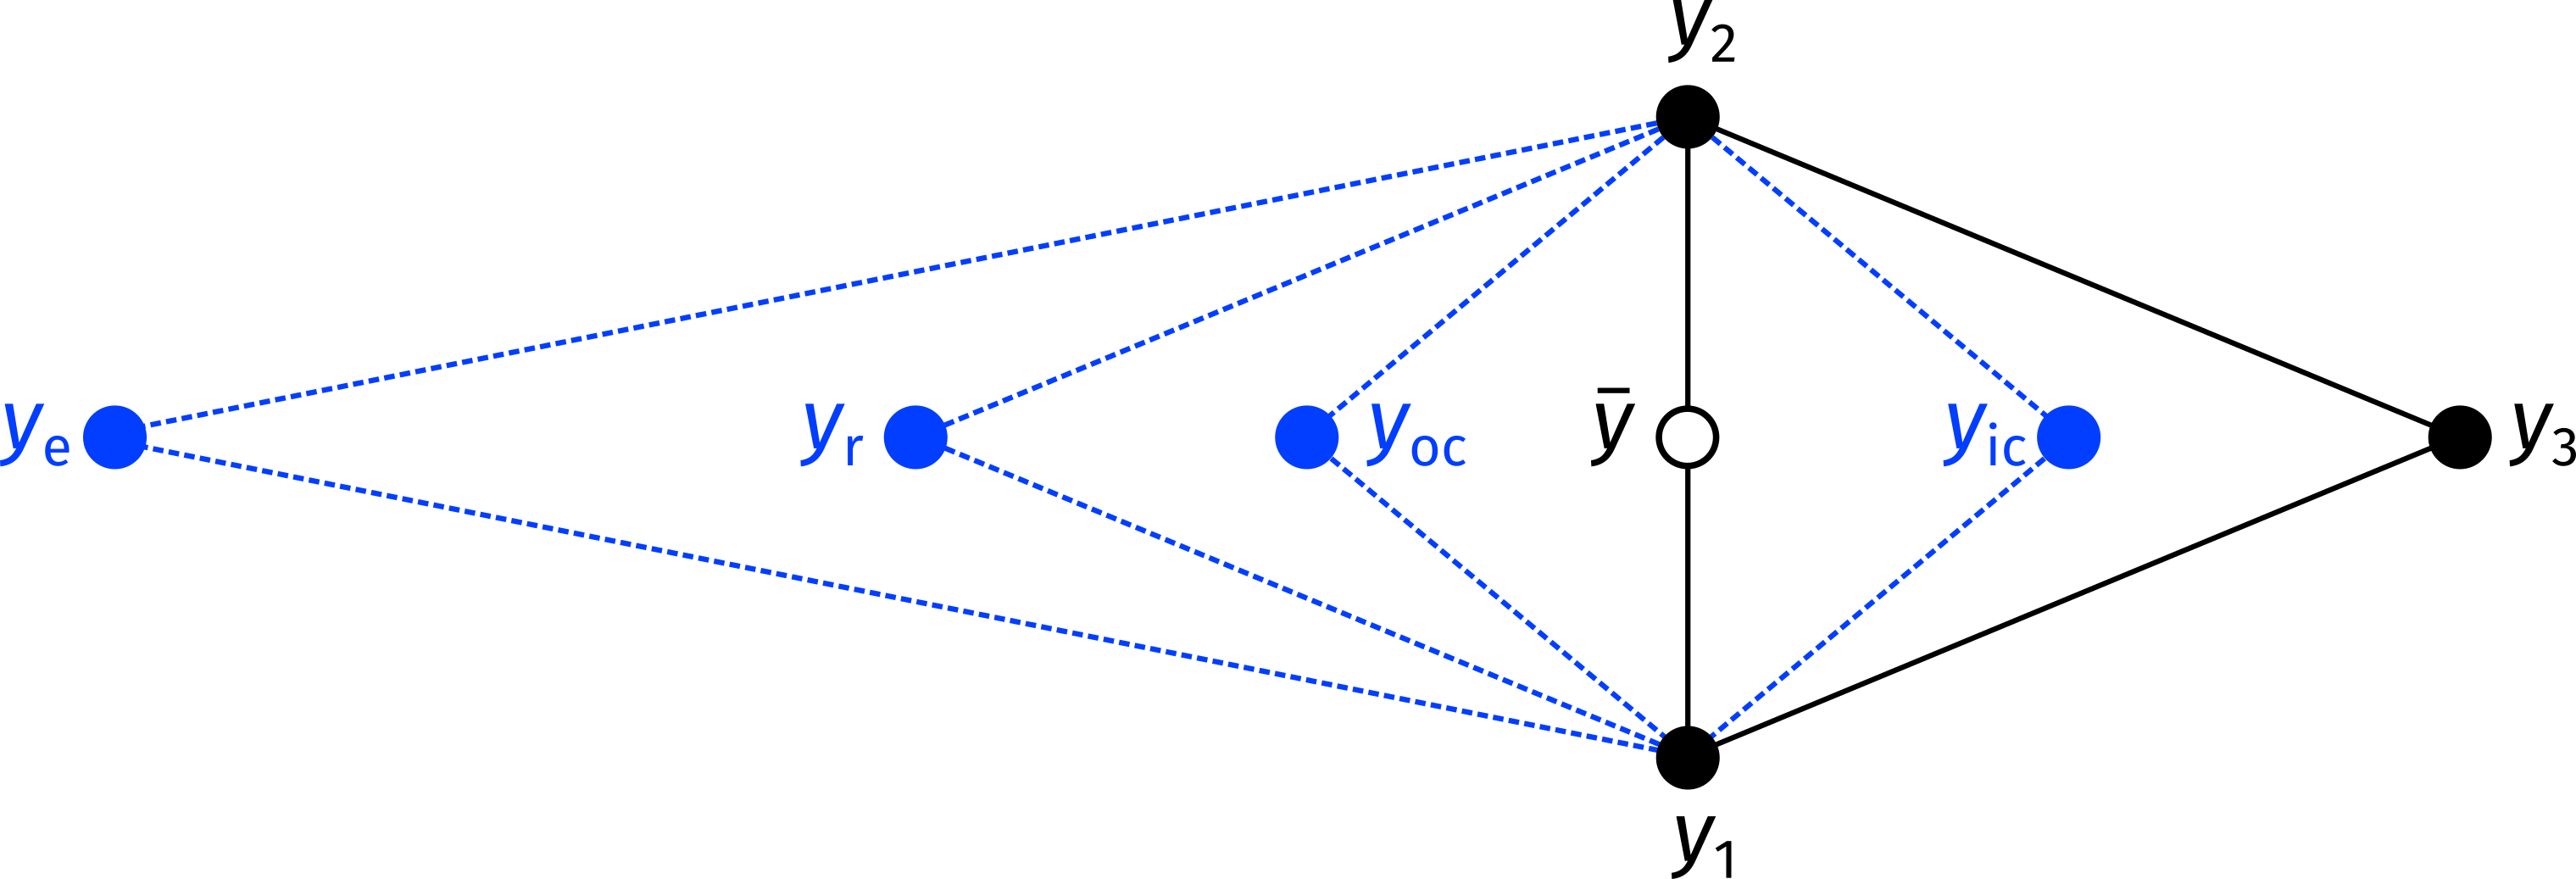
\includegraphics[]{poise/neldermead.png}%
    \caption[Trial points in an iteration of the Nelder--Mead algorithm]{
        Diagram showing various points evaluated in one iteration of the Nelder--Mead algorithm (for an optimisation of two parameters).
        The solid black lines indicate the boundaries of the simplex, which is assumed to be ordered such that $y_1$ is the best point (has the lowest cost function value) and $y_3$ the worst.
        The current points in the simplex are shown as filled black cirles, and the centroid $\bar{y}$ as an empty black circles.
        The blue circles indicate the trial points which the algorithm attempts to replace $y_3$ with, and are further discussed in the text.
        Blue dashed lines indicate the simplex which would result if the corresponding trial point were accepted.
    }
    \label{fig:neldermead}
\end{figure}

The NM algorithm is in fact quite intuitive to understand.
The initial simplex is first constructed using the supplied initial point: POISE specifically uses the method of Spendley et al.\autocite{Spendley1962T} to construct a \textit{regular simplex}.
The optimisation itself begins by measuring the cost function $f\/$ at every point of the simplex, and sorting the points in ascending order of cost function values (i.e.\ from best to worst), such that $f(y_1) \leq f(y_2) \leq \cdots \leq f(y_{n+1})$.
The centroid of the simplex is defined by the $n$ best points:
\begin{equation}
    \label{eq:simplex_centroid}
    \bar{y} = \sum_{i=1}^n y_i.
\end{equation}
On each iteration of the NM algorithm, we attempt to replace the worst point $y_{n+1}$  with a better point (\cref{fig:neldermead}).
The search for the new point is performed in several steps: first, the worst point is \textit{reflected} about the centroid of the simplex to obtain a new point $y_\text{r}$:
\begin{equation}
    \label{eq:nm_reflect}
    y_\text{r} = \bar{y} - (y_{n+1} - \bar{y}).
\end{equation}
The value of the cost function is evaluated at this point, and is compared against the existing points in the simplex.
If this reflected point falls in the middle of the pack, such that $f(y_1) \leq f(y_\text{r}) < f(y_n)$, this represents a `modest' improvement in the cost function: we simply replace the worst point with this and continue to the next iteration.

On the other hand, if the reflected point is better than all the other points (i.e.\ $f(y_\text{r}) < f(y_1)$), then we ambitiously attempt to \textit{expand} the simplex even further in that direction:
\begin{equation}
    \label{eq:nm_expand}
    y_\text{e} = \bar{y} - 2(y_{n+1} - \bar{y}).
\end{equation}
Of course, there is no guarantee that this is necessarily better than $y_\text{r}$; therefore, we choose whichever point of $y_\text{r}$ or $y_\text{e}$ had a lower value of $f$, and replace the worst point with this and continue to the next iteration.

If the reflected point is an improvement on the worst point but is no better than the remaining points, in that $f(y_n) \leq f(y_\text{r}) < f(y_{n+1})$, then the algorithm performs an \textit{outside contraction}, which resembles a half-hearted reflection:
\begin{equation}
    \label{eq:nm_outside_contract}
    y_\text{oc} = \bar{y} - (1/2)(y_{n+1} - \bar{y}).
\end{equation}
Conversely, if the reflected point is even worse than the worst point, in that $f(y_{n+1}) \leq f(y_\text{r})$, then this suggests that that search direction is very poor: we thus perform an \textit{inside contraction}, which uses a point halfway between the worst point and the centroid:
\begin{equation}
    \label{eq:nm_inside_contract}
    y_\text{ic} = \bar{y} + (1/2)(y_{n+1} - \bar{y}).
\end{equation}
If either of these contracted points are any better than $y_\text{r}$, then we replace the worst point in the simplex and continue to the next iteration; otherwise, we conclude that no search direction was good, and simply shrink the simplex towards the current best point by replacing each point $y_k$ with $(y_k + y_1)/2$.
In practice, these `last-resort' shrink steps occur very rarely.

Finally, convergence is signalled when in every dimension of the optimisation, the width of the simplex is smaller than the chosen optimisation tolerance.%
\footnote{The implementation of the NM algorithm in the \texttt{scipy} library only accepts a single value for the `tolerance', which is then used in all dimensions.
This is designed to be used by scaling the parameters beforehand such that the tolerance in each dimension is equal (and in fact, POISE was later updated to do so).
However, during initial development I chose instead to re-implement the NM algorithm with a convergence check which allowed for different tolerances to be specified in each dimension.}
For a multiple-parameter optimisation, this can potentially mean that extra accuracy is obtained in one of the parameters (because the simplex may have shrunk along that dimension more quickly).
However, it does guarantee that \textit{at least} the specified level of accuracy in every dimension is achieved.
